\documentclass{article}
\usepackage[portuguese]{babel}
\usepackage[square,numbers]{natbib}
\bibliographystyle{abbrvnat}
\usepackage{url}
\usepackage{pdfpages}
%\usepackage[table,xcdraw]{xcolor}
\usepackage{amsmath}
\usepackage{graphicx}
\usepackage{listingsutf8}
\graphicspath{{images/}}
\usepackage{parskip}
\usepackage{fancyhdr}
\usepackage{vmargin}
\usepackage{float}
\usepackage{caption}
\usepackage{subcaption}
\usepackage{hyperref}
\usepackage{listings}
\usepackage{pdfpages}
\usepackage{bytefield}
\usepackage{array} 
\usepackage{xparse}
\usepackage{tikz}
\usepackage{verbatim}
\usepackage{arydshln}
\usepackage{mathtools}
\usepackage{booktabs}
\usepackage{tabulary,lipsum}
\usepackage{svg}
\usepackage{pdflscape}
\usepackage{minted}
\usepackage{multirow}
\usepackage{fancyhdr}
\pagestyle{fancy}

\tymin=60pt
\tymax=\maxdimen

\setminted{
fontsize=\large,
breaklines,
breakbytoken=false,
breakautoindent=true,
baselinestretch=1.0,
framesep=2mm,
numbersep=2mm,
linenos,
frame=leftline
}

\renewcommand{\theFancyVerbLine}{\sffamily \textcolor[rgb]{0,0,0}{\large {\arabic{FancyVerbLine}}}}


\newcommand{\sectionbreak}{\clearpage}


\newcommand{\tikzb}[1]{\newsavebox{\#1}}

\setmarginsrb{3 cm}{2.5 cm}{3 cm}{2.5 cm}{1 cm}{1.5 cm}{1 cm}{1.5 cm}


\setlength\parindent{24pt}


\NewDocumentCommand{\codeword}{v}{%
\texttt{\textcolor{codelaranja}{#1}}%
}
\NewDocumentCommand{\redword}{v}{%
\texttt{\textcolor{red}{#1}}%
}
\NewDocumentCommand{\greenword}{v}{%
\texttt{\textcolor{green}{#1}}%
}

\NewDocumentCommand{\blueword}{v}{%
\texttt{\textcolor{blue}{#1}}%
}

\NewDocumentCommand{\majentaword}{v}{%
\texttt{\textcolor{majenta}{#1}}%
}

\usepackage[framed,numbered]{matlab-prettifier}
\lstset{
  style      = Matlab-editor,
  basicstyle = \fontfamily{pcr}\selectfont\footnotesize, % if you want to use Courier
}

\lstdefinelanguage{C2}[]{C}{
    %morestring = [s][\color{codelaranja}]{  <}{>},
}

\lstdefinestyle{mystyle}{
    backgroundcolor=\color{backcolour},   
    commentstyle=\color{codegreen},
    keywordstyle=\color{AzulTop},
    numberstyle=\tiny\color{codegray},
    stringstyle=\color{codelaranja},
    basicstyle=\ttfamily\footnotesize,
    breakatwhitespace=false,         
    breaklines=true,                 
    captionpos=b,                    
    keepspaces=true,                 
    numbers=left,                    
    numbersep=5pt,                  
    showspaces=false,                
    showstringspaces=false,
    showtabs=false,                  
    tabsize=2,
}

\definecolor{codegreen}{rgb}{0,0.6,0}
\definecolor{codegray}{rgb}{0.5,0.5,0.5}
\definecolor{codelaranja}{rgb}{0.93,0.6,0.32}
\definecolor{backcolour}{rgb}{0.95,0.95,0.92}
\definecolor{AzulTop}{rgb}{0.3,0.55,0.94}
\definecolor{LightCyan}{rgb}{0.88,1,1}
\definecolor{blue}{rgb}{0,0,1}
\definecolor{green}{rgb}{0,1,0}
\definecolor{red}{rgb}{1,0,0}
\definecolor{majenta}{rgb}{1,0,1}
\lstset{
    style=mystyle, 
    inputencoding=utf8,
    extendedchars=true,
    literate={á}{{\'a}}1 {à}{{\`a}}1 {ã}{{\~a}}1  {Ã}{{\~A}}1 {â}{{\^a}}1 {é}{{\'e}}1 {ê}{{\^e}}1 {ë}{{\"e}}1 {í}{{\'i}}1 {ç}{{\c{c}}}1 {Ç}{{\c{C}}}1 {õ}{{\~o}}1 {ó}{{\'o}}1 {ô}{{\^o}}1 {ú}{{\'u}}1
}


\lstdefinestyle{DOS}
{
    backgroundcolor=\color{black},
    basicstyle=\scriptsize\color{white}\ttfamily
}

\title{Relatório do Laboratório 7}								% Title
\author{} %<------------------------------------------------------								% Author
\date{\today}											% Date

\makeatletter
\let\thetitle\@title
\let\theauthor\@author
\let\thedate\@date
\makeatother

\pagestyle{fancy}
\fancyhf{}
\rhead{\theauthor}
\lhead{\thetitle}
\cfoot{\thepage}


\ifpdf
  \DeclareGraphicsRule{*}{mps}{*}{}
\fi

\begin{document}

%%%%%%%%%%%%%%%%%%%%%%%%%%%%%%%%%%%%%%%%%%%%%%%%%%%%%%%%%%%%%%%%%%%%%%%%%%%%%%%%%%%%%%%%%

\begin{titlepage}
	\centering
    \vspace*{0.2 cm}
    
\includegraphics[scale = 0.8]{logoPoli.jpg}\\[1.0 cm]	% University Logo
    \textsc{\LARGE \newline\newline Escola Politécnica da USP}\\[1.5 cm]	% University Name
    \textsc{\Large PMR3406 - Microprocessadores em Automação e Robótica}\\[0.5 cm] %Course Code     
    \textsc{\Large Turma 03 - Grupo 02}\\[0.5 cm]
	
	\rule{\linewidth}{0.2 mm} \\[0.4 cm]
	{ \huge \bfseries \thetitle}\\ 
	\rule{\linewidth}{0.2 mm} \\[1 cm]
	
	\begin{minipage}{0.5\textwidth}
		\begin{flushleft} \large

            Antônio Augusto Carnevalli\\
			Thiago Lam Braweman\\

			
			\end{flushleft}
	\end{minipage}~
	\begin{minipage}{0.5\textwidth}
            
		\begin{flushright} \large

            13682909\\
			10770502\\

		    
		    \end{flushright}
        
	\end{minipage}\\~
	\vfill
	\thedate
	
    
\end{titlepage}


% (1)---------------------------------------------------------------------------------
\section{Solução do problema proposto}
% Texto explicativo sobre como resolver o problema da tarefa proposta.
Nessa atividade foi implementada uma lógica de funcionamento para um robô seguidor de linha, utilizando a PIC16F886. Para tanto, o roteiro do laboratório estabelece alguns requisitos:
\begin{enumerate}
  \item Uma chave deve ser pressionada para o robô iniciar a tarefa
  \item O LED RGB deve mudar de cor de acordo com o movimento do robô
  \item O LED deve sinalizar a cor vermelha ao encontrar um obstáculo
\end{enumerate}
O robô conta com um conjunto de três sensores do tipo infravermelho, que faz leituras e retorna sinais 0 ou 1 de acordo com a luminosidade observada. Além disso, também conta com um sensor analógico de proximidade frontal.

Para resolver o problema estabelecido, a velocidade da roda deve ser ajustada com base na leitura dos 3 bits do sensor de linha, de modo a manter a linha de fita preta alinhada com o sensor central. O sensor central deve detectar se há algum obstáculo à frente, parando o robô caso necessário. Se não for detectada nenhuma linha preta (todos os sensores retornam 0), o robô deve executar um movimento circular até encontrar uma linha novamente.
De forma geral, a solução consiste em adotar rotinas de execução de ações com base nas leituras dos sensores de linha e proximidade.
% (2)---------------------------------------------------------------------------------
\section{Funcionamento do programa}

% Texto explicativo sobre o funcionamento do programa. Incluir condições nas quais que
% são sinalizadas no LED RGB.

O programa pode ser dividido em 2 partes, as \textbf{Entradas} (Chave, sensor de proximidade e sensor de linha) e as \textbf{Saídas} (PWM e LED\_RGB).

\subsection{Chave}

A chave é utilizada como um botão, mudando o estado do robô de ligado para desligado e vice-versa, ela é iniciada como desligada.\par 
Assim como nos laboratórios utilizamos a biblioteca "key.h" e Interrupt-On-Change na porta B para ler o estado da chave.\par

\begin{lstlisting}[style = Matlab-editor, language = C2]
#include "key.h"
    ...
if (RBIE && RBIF) { // se for mudança estado do Port B        
    char portB = PORTB; // faz a leitura do Port B
    key_read(portB);    // faz a leitura da chave
    RBIF = 0;           // reseta o flag de interrupção 
} // fim - tratamento I-O-C PORT B
\end{lstlisting}

Na função \codeword{main} do programa criamos 2 vaiáveis \codeword{keyIn} e \codeword{isOn}, ambas são do tipo \codeword{char}. A variável \codeword{keyIn} é iniciada com valor FALSE (ou 0), ela nos informa se a chave foi pressionada. A variável \codeword{isOn} é iniciada com o valor OFF (ou 0), ela nos informa o estado do robô (ligado ou desligado). Antes de entrar no loop principal ainda devemos iniciar a chave usando a função \codeword{key_init()}.\par

\begin{lstlisting}[style = Matlab-editor, language = C2]
char keyIn = FALSE; // tecla pressionada, TRUE = sim
char isOn = OFF;    // modo autônomo, inicialmente desligado
...
key_init();         // inicializa chave
\end{lstlisting}

Dentro do loop principal criamos um \codeword{if} que é chamado quando a chave for pressionada, dentro desse condicional a variável \codeword{isOn} é invertida, se estivesse em 1 ia para 0, e se estivesse em 0 ia para 1.\par
Mais a frente no loop principal colocamos dois condicionais \codeword{if} para distinguir os estados ligado e desligado. (Não usamos \codeword{else} para facilitar a leitura)

\begin{lstlisting}[style = Matlab-editor, language = C2]
// liga ou desliga o robô
if (keyIn){
    isOn = ~isOn;       // muda o estado
    beep();             // para debug
    LED =  (__bit)isOn; // para debug
} // Fim do if(keyIn)

if(!isOn){  // se estiver desligado
    ...
} // Fim do if(!isOn)

if(isOn){   // se estiver ligado
    ...
} // Fim do if(isOn)
\end{lstlisting}

\subsection{Sensor de Proximidade}
O sensor de proximidade é utilizado para evitar colisões do robô, a partir dele a velocidade deve ser controlada (quanto mais perto menor a velocidade), chegando a parar à uma certa distância predefinida. (Obs. o valor digital do sensor aumenta quanto menor a distância e se aproximando a 0 quanto mais longe)\par

\begin{lstlisting}[style = Matlab-editor, language = C2]
// caso a distância seja menor ou igual a mínima
if (nearSensorData >= DIST_THRESHOLD ){     
    // para o robô 
    ...
} else{
    // ajusta a velocidade
    dutyCycle = 600 - nearSensorData;
    ...
}
\end{lstlisting}

Para utilizar o sensor de proximidade importamos a biblioteca \codeword{sensor.h}, iniciamos (dentro do main) os sensores com \codeword{sensor_init()}, criamos uma variável (int) local \codeword{nearSensorData}, e por fim utilizando a função \codeword{sensorNear_read()} e conseguimos ler o valor digital (graças ao ADC).\par


\begin{lstlisting}[style = Matlab-editor, language = C2]
#include "sensor.h"

void main (void){       // Programa Principal
    int nearSensorData; // valor do sensor de proximidade
    sensor_init();      // inicializa sensores
    ...
    while(1){           // Loop Principal
        nearSensorData = (int)sensorNear_read();    // salva o valor do sensor de proximidade
        ...
    } // Fim do Loop Principal
} // Fim do Programa Principal
\end{lstlisting}



\subsection{Sensor de Linha}

O sensor de linha é responsável pela funcionalidade de seguir linha do robô, ele informa o robô a posição das marcações pretas na pista. O sensor é composto por 3 sensores ópticos em linha e espaçados em 9,5 mm que detectam se a faixa preta esta em baixo deles. Sua saída então é um valor de 0 à 7 que representas os estados abaixo. 

\begin{figure}[H]
    \centering
    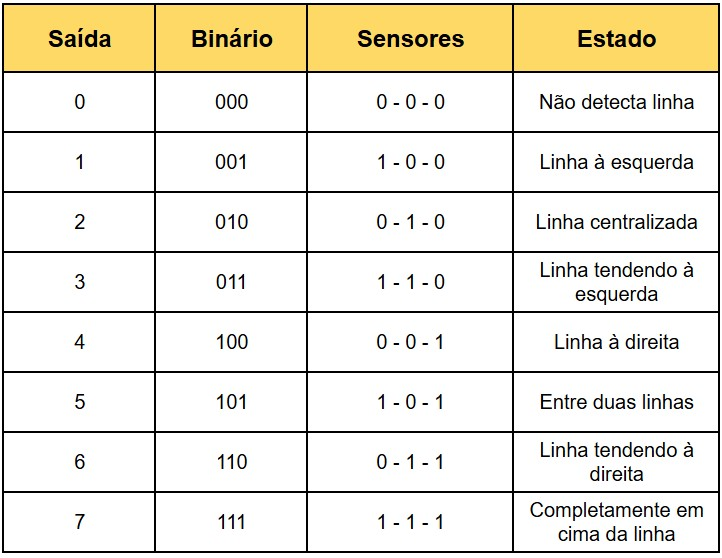
\includegraphics[width = .8\linewidth]{images/EstadosLinha.jpg}
    \caption{Tabela de saídas do sensor de linha.}
    \label{tab:estadosLinha}
\end{figure}

Para utilizar o sensor de linha devemos importar a biblioteca \codeword{sensor.h}, no programa principal criamos uma variável \codeword{lineSensor} para armazenar o valor lido e iniciamos o sensor com o comando \codeword{sensor_init()}. Finalmente podemos fazer a leitura do sensor com o comando \codeword{sensorLine_read()}.

\begin{lstlisting}[style = Matlab-editor, language = C2]
#include "sensor.h"

void main (void){       // Programa Principal
    union chartype lineSensor;  // valor do sensor de linha
    sensor_init();      // inicializa sensores
    ...
    while(1){           // Loop Principal
        lineSensor.byte = sensorLine_read(); // valor do sensor de linha
        ...
    } // Fim do Loop Principal
} // Fim do Programa Principal
\end{lstlisting}

Na lógica do programa dividimos em categorias as leituras do sensor de linha baseado nas ações que o robô deveria tomar, andar para frente (saídas 2, 5 e 7), girar no sentido horário (saídas 1 e 3), girar no sentido anti-horário (saídas 4 e 6) e rodar em um círculo (saída 0).

\begin{lstlisting}[style = Matlab-editor, language = C2]          
// estados do sensor de linha (0 - 7)
switch (lineSensor.byte){
    case 7: // sensor de linha : 1-1-1
    case 2: // sensor de linha : 0-1-0
    case 5: // sensor de linha : 1-0-1
                            
        // Andar em linha reta
        pwm_set(1,dutyCycle - 200);     // motor esquerdo em velocidade média
        pwm_set(2,dutyCycle - 200);     // motor direito em velocidade média
        led_rgb_set_color(2);           // LED RGB cor verde
        break;

    case 4: // sensor de linha : 0-0-1               
    case 6: // sensor de linha : 0-1-1
                            
        // Girar sentido horário
        pwm_set(1,dutyCycle - 200);     // motor esquerdo em velocidade média
        pwm_set(2,dutyCycle - 400);     // motor direito em velocidade baixa
        led_rgb_set_color(1);           // LED RGB cor azul
        break;

    case 1: // sensor de linha : 1-0-0
    case 3: // sensor de linha : 1-1-0
                            
        // Girar sentido anti horário
        pwm_set(1,dutyCycle - 400);     // motor esquerdo em velocidade alta 
        pwm_set(2,dutyCycle - 200);     // motor direito em velocidade média
        led_rgb_set_color(5);           // LED RGB cor magenta
        break;

    case 0: // sensor de linha : 0-0-0
                            
        // Rodar em círculo no sentido horário
        pwm_set(1,dutyCycle -100);      // motor esquerdo em velocidada alta
        pwm_set(2,dutyCycle - 300);     // motor direito em velocidade média
        led_rgb_set_color(1);           // LED RGB cor azul
        break;

    default: // Outras entradas
                            
        // para o robô
        pwm_set(1,0);           // motor esquerdo parado
        pwm_set(2,0);           // motor direito parado
        break;
} // Fim do switch
\end{lstlisting}

\subsection{PWM}
O PWM é utilizado para mover o robô, caso precise parar, andar em linha reta, girar em um sentido ou fazer um círculo. Quando for necessário parar o duty cycle dos dois motores são 0. Para seguir em frente o duty cycle deve se um valor maior que 0 e ser igual em ambos os motores. Para girar deve existir uma diferença entre os duty cicles dos motores, ao girar em círculos essa diferença não deve muito grande, assim criando um raio maior. Para fazer curvas a diferença entre os duty cycles deve ser mais expressiva e o sentido do giro é determinado pela escolha dos motores, no sentido horário o esquerdo é mais rápido que o direito e no anti horário o inverso.\par

Quanto implementação do PWM utilizamos a função \codeword{pwm_set()} desenvolvida para o laboratório 6 (\codeword{pwm.c}), com ela conseguimos escolher o canal 1 ou 2 (motor esquerdo ou direito) e ajustamos o valor do duty cycle (0 - 1000). Como os motores só suportam cerca de 60\% da carga, os valores devem estar no intervalo de 0 - 600.

\begin{lstlisting}[style = Matlab-editor, language = C2]
#include "pwm.h"
...
// girando no sentido horário
pwm_set(1,500);   // ajusta o PWM do motor esquerdo
pwm_set(2,200);   // ajusta o PWM do motor direito
\end{lstlisting}



\subsection{LED RGB}

O LED RGB deve funcionar como um indicativo para o estado do robô, desligado quando o robô estiver desligado, \redword{vermelho} quando o robô estiver muito próximo de um obstáculo (parado), \greenword{verde} se estiver indo em linha reta, \blueword{azul} se estiver girando no sentido horário \majentaword{magenta} se estiver indo no sentido anti-horário.\par

Para utilizar o LED RGB devemos incluir a biblioteca \codeword{led_rgb.h}, dentro do \codeword{main} iniciamos o ela com a função \codeword{led_rgb_init()} e depois ajustamos a cor com a função \codeword{led_rgb_set_color(x)} onde x é um valor de 0 à 7 que representa 8 cores diferentes.  

\begin{lstlisting}[style = Matlab-editor, language = C2]
#include "led_rgb"
...
void main(void){
    led_rgb_init();             // inicializa o LED RGB
    ...
    while(1){
        led_rgb_set_color(1);   // LED RGB cor azul
        ...
    }
}
\end{lstlisting}

(Obs. O LED verde da nossa placa estava queimado, então não conseguimos verificar a cor verde, mas as outras foram testadas).
% (3)---------------------------------------------------------------------------------
\section{Discussão dos objetivos}
% Discutir até que ponto os objetivos foram alcançados.
Ao final do laboratório, foram atingidos os seguintes objetivos: 

O carrinho funcionava ao apertar o botão de start, seguindo normalmente a linha da fita e ajustando a velocidade e orientação quando necessário. 

O sensor de proximidade também funcionou com sucesso, reduzindo e parando conforme a distância aferida. Os LEDs também trocavam de cor conforme o estabelecido pelo roteiro, com exceção do LED de cor verde, pois este estava com defeito no dispositivo fornecido pela disciplina para este laboratório, estando aparentemente queimado. Mesmo não funcionando, acredita-se que também funcionaria com o código desenvolvido, pois segue a mesma lógica de acionamento das demais cores.

Um detalhe que não foi possível confirmar o funcionamento foi o botão de parada. O robô iniciava ao apertar o botão, mas depois não parava quando acionado o botão novamente. Foram testadas várias hipóteses, e mesmo chamando o professor para auxiliar, o mesmo também não conseguiu apontar o que poderia estar errado, pois o código aparentemente estava correto.

\newpage
% (4)---------------------------------------------------------------------------------
\section{Código fonte}
% Código fonte com comentários explicando o funcionamento do programa. Incluir somente
% os programas que foram escritos para essas atividades.

\inputminted{c}{code/code.c}

\end{document}